\chapter{The proposed architecture}
\label{chap:met}
\lstdefinestyle{customc}{
    belowcaptionskip=1\baselineskip,
    breaklines=true,
    frame=L,
    xleftmargin=\parindent,
    language=C,
    showstringspaces=false,
    basicstyle=\footnotesize\ttfamily,
    keywordstyle=\bfseries\color{mymauve},
    commentstyle=\itshape\color{mygreen},
    identifierstyle=\color{blue},
    stringstyle=\color{orange},
    numbers=left,
    captionpos=b
}
  
\lstset{escapechar=@,style=customc}

Authors of the language propose the following pipeline of the compilation of software written in SLang (Figure \ref{fig:compiler_pipeline}). The compiler starts with a parser which parses the source code in SLang into an AST, for it to be then converted into a kind of intermediate representation, which is further converted to a target platform code.

\begin{figure}[h!]
    \centering
    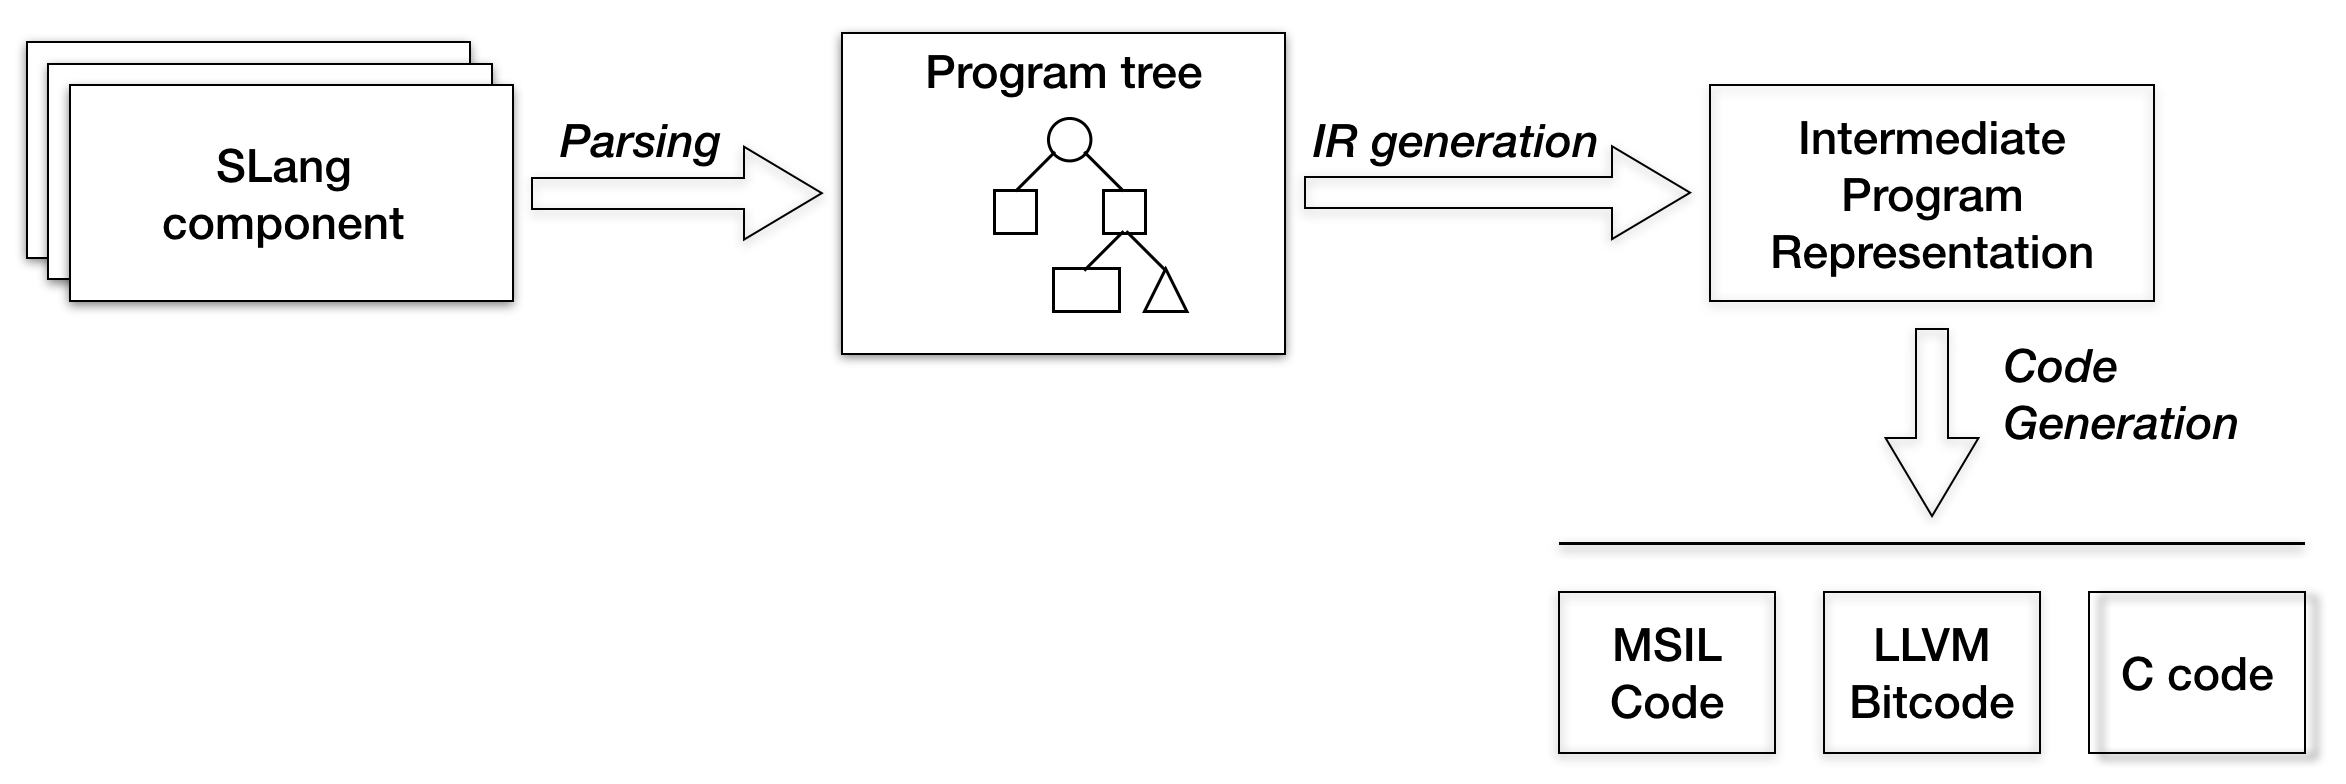
\includegraphics[width=\linewidth]{compiler_pipeline.png}
    \caption{Compiler pipeline}
    \label{fig:compiler_pipeline}
\end{figure}

As a part of a process of the compiler development, three kinds of platforms are proposed to perform code generation into, namely .NET, LLVM and C language. In this work, implementation of code generation in C is developed. This decision is motivated by the fact that multiple architectures existing nowadays have a C compiler written for them, which includes proprietary like Elbrus \cite{Elbrus} or for embedded systems which only have a C or assembler compiler.

\section{Compiler frontend, middle-end and backend}
The notion of a modern compiler implies modularity, or division into modules, which include frontend, backend and sometimes middle-end. This way of structuring allows dividing compiler development into language syntax description, code generation for specific hardware and optimization respectively, which, in its turn, proved to help to simplify both the process of compiler development and the process of it being expanded by third-party developers.

With modular compiler architecture, a developer of a new language needs to describe the syntax and rules of translation of language constructs into some high-level representation constructs, instead of caring about how these constructs are implemented on the low level in any particular architecture.

In other words, modularity allows developers to reuse already existing components to expand language-platform variety, which led to compilers designed this way being called retargetable.

On the picture described above (Fig \ref{fig:compiler_pipeline}), the front-end is the parser, the middle-end consists of IR generation and code generation, and backend is necessarily the target platform, for which code generation is performed.

As we need to find out how to make a system that works, it is necessary to review existing works in the field. In this section, we will mostly concentrate on two most popular open source compilers, namely GCC and LLVM, due to them being actively developed by open source community and incredibly widely used, which implies they are reliable enough to be exemplary.
 

\subsection{Compiler frontend}
The compiler frontend is a part of a compiler translating source code to some intermediate representation. 
Usually, frontend pipeline includes some or all of the following steps in the specified order:
\begin{enumerate}
    \item \textbf{Lexical analysis}
    \begin{itemize}
        \item \textbf{Line reconsruction} changes strings of literals into a parser-suitable format, usually deleting comments, tabulations, unnecessary spacing and new line characters;
        \item \textbf{Preprocessing} applies macros or others built-in language preprocessing functions; 
        \item \textbf{Tokenization} breaks the preprocessed code into lexical tokens, which can be interpreted by compiler to construct IR;
    \end{itemize}
    \item \textbf{Syntax analysis} parses the set of tokens into an \textit{abstract syntax tree (AST)} or other type of IR;
    \item \textbf{Semantic analysis} adds metainformation to IR tokens, such as type or access modifiers, and performs error checking; 
\end{enumerate}

GCC, for instance, provides frontends for C, C++, Objective-C, Fortran, Ada, and Go languages \cite{GNU}, while LLVM can use frontends based on the GCC 4.2 parsers as well as its frontends \cite{LLVM_features}.

\subsection{Compiler middle end (ordinary optimizer)}

This step performs optimizations on the IR level. The advantage of it is that powerful optimizers do not usually allocate memory until optimization is performed, and only do it when it is clear that individual variables do not exist outside registers, so they do not need memory allocation. Moreover, it makes possible to determine the order in which variables are to be allocated in memory so that maximal amount of them is cached, which, in its turn, positively affects performance.

\subsubsection{GCC}
GCC middle-end is explicitly defined and performs SSA-based\footnote{\textbf{Static Single Assignment form (SSA)} is a property of an IR, which requires that each variable is assigned exactly once, and every variable is defined before it is used. \cite{SSA_wiki} } optimizations of a program translated to GIMPLE (one of a few intermediate representations in GCC), and then translates GIMPLE into RTL\footnote{\textbf{Register Transfer Language (RTL)} is a kind of intermediate representation (IR) that is very close to the assembly language, such as that which is used in a compiler. \cite{RTL_wiki}}, where more low-level optimizations are performed, and then, after it is done, the optimized program in RTL is redirected to compiler back-end.

\subsubsection{LLVM}
In LLVM, middle-end is explicitly defined as well and is utilized to translate the program into an intermediate language called bit code language, perform SSA optimizations in bit code, and redirect the program to back-end afterward.

\subsubsection{SLang}
This step will perform optimizations and construct data structures for the C language, as C, for example, does not have classes as language constructs, which implies the need to represent them as sets of structures and functions related to them.

\subsection{Compiler backend}
The backend is a part of a compiler which generates code and performs optimizations for a specific CPU architecture.

\begin{itemize}
    \item \textbf{LLVM} supports multiple architectures, including X86, X86-64, and ARM. The full list is available on the LLVM website \cite{LLVM_features};
    \item \textbf{GCC} is older than LLVM and supports more architectures. The list of all supported architectures is presented on the GCC website \cite{GCCback};
\end{itemize}


\section{Abstract Syntax Tree (AST)}
AST is a way to represent a program in a tree form. Each node of AST denotes a construct occurring in the source code, written in a programming language. The tree is called abstract since not all syntactic details are preserved. Because of that, programs written in different programming languages but doing the same thing may well have the same AST structure.

Since one of the objectives of this thesis is the design of AST representation, let us now look at what options exist presently.

\subsection{Variants of representation}

Consider AST for GCC and LLVM:
\begin{itemize}
    \item \textbf{GCC} allows us to get plenty of variants of program representation. Using the command ``gcc-7 test.c -fdump-tree-all'', it is possible to generate many files that appear in the course of performing optimizations. One of them is a ``.gimple'' file that contains the code of a program in GIMPLE language, Listing \ref{lst:GCC_gimple}. In an ``.optimized'' file, Listing \ref{lst:GCC_gimple_optimized}, there is an optimized version of the code in GIMPLE.

    \item In \textbf{LLVM}, CLang is a part of LLVM toolchain, or, to be more specific, the compiler frontend for C, C++ and Objective-C programming languages \cite{CLangDoc}. 
    CLang contains a part responsible for AST construction, which uses the kind of AST that slightly differs from those used in other compilers, for it to resemble C++ code structure, for instance, ``parenthesis expressions and compile-time constants are available in an unreduced form in the AST'' \cite{CLangAST}.
    This feature makes CLang AST more suitable for refactoring tools.
\end{itemize}

Consider the following program in C:
\begin{lstlisting}[caption={Example of a C source code}, label=lst:C_Example]
    // test.c
    int main() {
        int a = 1; 
        int b = 2;
        return a + b;
    }
\end{lstlisting}

Obviously, this program can be optimized into call of \textit{return 3;} in the \textit{main} function. Let us now consider the ways of this program being optimized by two compilers mentioned above.


In Clang, we can output the AST representation of a program to the terminal. For the previous example, the tree looks as follows:

\begin{lstlisting}[morekeywords={FunctionDecl, CompoundStmt, DeclStmt, VarDecl, IntegerLiteral, ReturnStmt, TranslationUnitDecl, ImplicitCastExpr, DeclRefExpr}, caption={CLang AST}, label=lst:CLang_AST]
    $ clang -Xclang -ast-dump -fsyntax-only test.c

    TranslationUnitDecl 0x5aea0d0 <<invalid sloc>>
    ... cutting out internal declarations of clang ...
    `-FunctionDecl 0x7ff950058400 <test.c:1:1, line:6:1> line:1:5 main 'int ()'
    `-CompoundStmt 0x7ff950058740 <col:11, line:6:1>
      |-DeclStmt 0x7ff950058570 <line:2:1, col:10>
      | `-VarDecl 0x7ff9500584f0 <col:1, col:9> col:5 a 'int' cinit
      |   `-IntegerLiteral 0x7ff950058550 <col:9> 'int' 1
      |-DeclStmt 0x7ff950058620 <line:3:1, col:10>
      | `-VarDecl 0x7ff9500585a0 <col:1, col:9> col:5 b 'int' cinit
      |   `-IntegerLiteral 0x7ff950058600 <col:9> 'int' 2
      |-DeclStmt 0x7ff9500586d0 <line:4:1, col:10>
      | `-VarDecl 0x7ff950058650 <col:1, col:9> col:5 used c 'int' cinit
      |   `-IntegerLiteral 0x7ff9500586b0 <col:9> 'int' 3
      `-ReturnStmt 0x7ff950058728 <line:5:1, col:8>
        `-ImplicitCastExpr 0x7ff950058710 <col:8> 'int' <LValueToRValue>
          `-DeclRefExpr 0x7ff9500586e8 <col:8> 'int' lvalue Var 0x7ff950058650 'c' 'int'
\end{lstlisting}


% \begin{lstlisting}[frame=L, numbers=left, language=C, basicstyle=\footnotesize, caption=GCC AST\label{lst:GCC_AST}]
% gcc tree
% \end{lstlisting}
% [discription]

Both compilers allow us to have a look at IR and observe opimizations being done. Here is how the bitcode looks fot the AST above:
%Оба компилятора позволяют рассмотреть IR и понаблюдать за проходками оптимизации этой программы:

\begin{lstlisting}[escapeinside={\%*}{*)}, caption={LLVM bitcode in SSA form}, label={lst:LLVM_bitcode}]
    $ clang -c -emit-llvm test.c -o test.bc
    $ llvm-dis test.bc -o test.ll // SSA
    $ clang -S -emit-llvm test.c -o test.ll

    ; ModuleID = 'test.c'
    define i32 @main() #0 {
        %1 = alloca i32, align 4
        %2 = alloca i32, align 4
        %3 = alloca i32, align 4
        store i32 0, i32* %1, align 4
        store i32 1, i32* %2, align 4
        store i32 2, i32* %3, align 4
        %4 = load i32, i32* %2, align 4
        %5 = load i32, i32* %3, align 4
        %6 = add nsw i32 %4, %5
        ret i32 %6
      }
\end{lstlisting}

The bitcode in the listing above is generated in SSA form. The @ prefix denotes global identifiers like function names, the \# symbol serves as a prefix for a code block ID, and the \% symbol denotes local identifiers like variable declarations. In this listing, memory allocation blocks are explicitly observable, as well as assignments and loading of assigned values to further use them to compute and return the result.

The GIMPLE code is more similar to C, compared to bitcode. For instance, in the listing \ref{lst:GCC_gimple} it is possible to find variable definition and declaration that looks just like in C.

\begin{lstlisting}[frame=L, language=C, numbers=left,basicstyle=\footnotesize, caption={GCC gimple in SSA form}, label={lst:GCC_gimple}]
    $ gcc-7 test.c -fdump-tree-all
    $ cat test.c.049t.ssa

    ;; Function main (main, funcdef_no=0, decl_uid=1809, cgraph_uid=0, symbol_order=0)
    
    main ()
    {
      int b;
      int a;
      int D.1814;
      int _3;
    
      <bb 2> [0.00%]:
      a_1 = 1;
      b_2 = 2;
      _3 = a_1 + b_2;
    
    <L0> [0.00%]:
      return _3;
    }
\end{lstlisting}

Next, optimized bitcode:
%Далее, оптимизированный код в биткоде:
\begin{lstlisting}[escapeinside={\%*}{*)}, caption=LLVM bitcode optimized, label={lst:LLVM_bitcode_o}]
    $ clang -c -emit-llvm test.c -o test.bc -O1
    $ llvm-dis test.bc -o test.ll

    ; ModuleID = 'test.c'
    define i32 @main() local_unnamed_addr #0 {
        ret i32 3
      }
\end{lstlisting} 
By default, when trying to observe bitcode, one is getting it without optimization. If one wishes to see the optimized code, they will need to compile it with the -O1 flag. In the listing, it is easy to see that the program was minimized as much as possible, and all expressions that did not bring anything useful were cut out. Furthermore, there is one more optimization on the main function, namely the expression ``local\_unnamed\_addr'' being added before the function, which is described in the documentation as follows: ``If the ``local\_unnamed\_addr'' attribute is given, the address is known to not be significant within the module.'' \cite{LLVM_manual}


\begin{lstlisting}[frame=L, language=C, numbers=left,basicstyle=\footnotesize, caption={Release GCC gimple in SSA form}, label={lst:GCC_gimple_optimized}]
    $ gcc-7 test.c -fdump-tree-all -O1
    $ cat test.c.049t.release_ssa

    ;; Function main (main, funcdef_no=0, decl_uid=1809, cgraph_uid=0, symbol_order=0) (executed once)
    
    Released 3 names, 150.00%, removed 3 holes
    main ()
    {
      <bb 2> [100.00%]:
      return 3;
    }
\end{lstlisting}
As we can see, this example also shows full optimization. Moreover, it is worth noting that in GCC, three optimization flags -- -O1, -O2, and -O3 -- are available, to allow for different levels of optimization. In fact, there are many more optimization flags which all have the different meaning, described on the GCC website \cite{GCC_optimizations}.

\section{Intermediate representation}
The intermediate representation is closely connected to AST -- as it is also a way of program representation. Often, AST itself is a form of IR, and other compilers\cite{Non_AST_compilers} can even transform code into non-AST IR omitting the AST stage. 

\subsection{Expressions of IR}
\begin{itemize}
    \item \textbf{LLVM bitcode} mentioned above in examples \ref{lst:LLVM_bitcode} and \ref{lst:LLVM_bitcode_o}. It is a low-level language, similar to assembly language, but unlike assembler, bitcode is not platform-dependent, even though it allows for platform-specific low-level operations.

    \item \textbf{CIL}. Common Intermediate Language designed by Microsoft, and it is a part of the .NET framework. Also similar to assembly language, and is used to represent a program inside the .NET virtual machine.

    \item \textbf{GIMPLE} is GCC intermediate language, as mentioned above. It comes in two flavors: High-Level GIMPLE is a common IR for all GCC front-ends and is generated in the middle end, listing \ref{lst:GCC_gimple}, while Low-Level GIMPLE is generated from the High-Level GIMPLE with the help of control flow graph generated for this purpose. The program in Low-Level GIMPLE is then SSA-optimized, and after that, translated to RTL, which has Lisp-like syntax.

    \item \textbf{C programming language}. For Eiffel, Sather, Esterel, Haskell \cite{GlasgowHaskellCompiler}, Cython. C was chosen to be used as one of the intermediate languages for SLang.
\end{itemize}

\subsection{Advantages}
\begin{itemize}
    \item IR allows compilers to perform multiple passes of program optimization;
    \item IR is some abstraction; therefore it can be used for other languages and other compilers;
    \item IR allows as well as AST perform CPU independent optimizations;
\end{itemize}

% \subsection{Disadvantages}
% \begin{itemize}
%     \item It slows down compilation process;
%     \item In any case, IR imposes restrictions on the language frontend;
%     [EXAMPLE]
% \end{itemize}

\subsection{Auxiliary representations}
There is a number of auxiliary representations commonly used in compilers\cite{UMDIR}:
\begin{itemize}
    \item Abstract syntax tree (AST) --- representation of a program in a tree form;
    \item Control flow graph (CFG) --- a way of representing a program with a graph that describes all possible paths of program execution;
    \item Three-address code (TAC) --- is a most useful way for a compiler to optimize a program. Every instruction in TAC consists of three operands  -- this is the reason why TAC is called this way; %which three operands?
    \item Stack-based representation (SBR) --- is a lower level representation of TAC -- each command of TAC can be converted to a few commands of SBR. SBR has quite a simple syntax, but it is not human-readable; 
\end{itemize}

% \subsection{Restrictions}

\section{Concept}
In this research, the middle-level representation (MLR) of SLang is going to be considered.

MLR is a vital part of a translator, which translates language SLang constructs to corresponding C entities, without loss of functionality. 
As the result of research, the high-level architecture of MLR now consists of the following parts:

\begin{itemize}
    \item \textbf{IR to MLR.} In our case, IR is going to be a variation of AST, stored in a JSON file. On this stage, the AST is going to be converted into the internal representation of the developed translator.
    \item \textbf{MLR.} The internal representation itself, or a model that stores the program semantics, ready to be translated into the C source code. In fact, it is a key point of this thesis: creating a representation of a program suitable for direct translation to C, item-to-source, through de facto deserialization of MLR objects into the C code (see fig \ref{fig:plan})
    \item \textbf{MLR to C.} On this stage, serialization of MLR into C is performed.
%На данном этапе происходит сериализация MLR в C.
\end{itemize}
At the figure \ref{fig:plan} the place of MLR in the process chain is shown.  

% \subsection{Existing solutions}
% [write about \cite{Necula2002}]
\begin{figure}[h!]
    \centering
    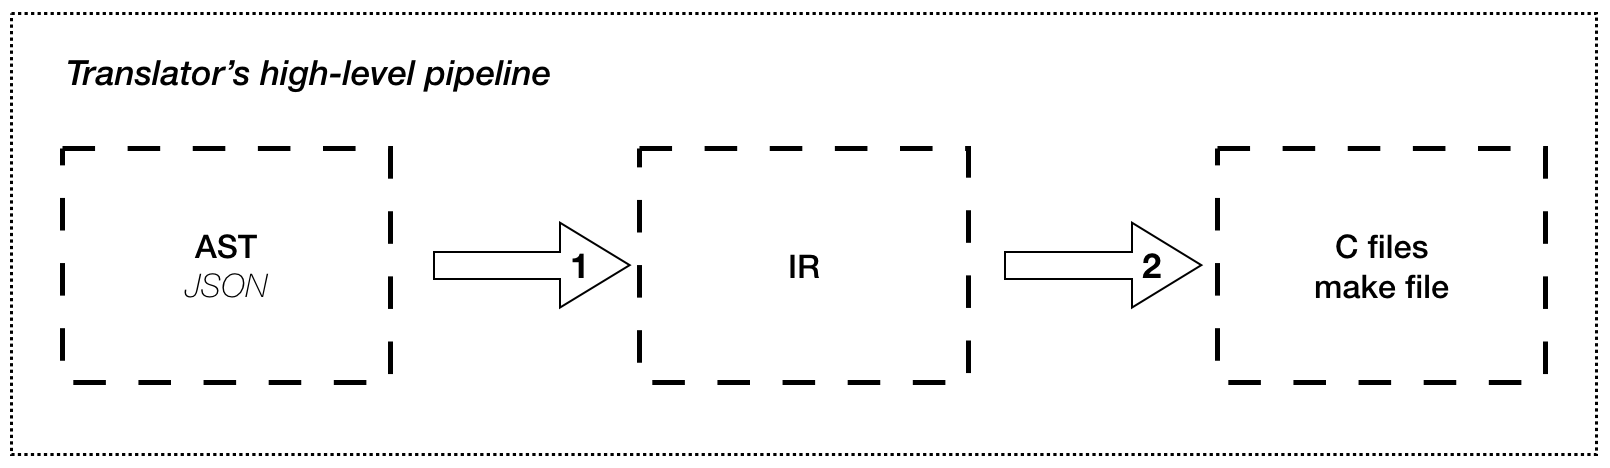
\includegraphics[width=\linewidth]{Translators_high_level_pipeline.png}
    \caption{Translator high-level pipeline}
    \label{fig:plan}
\end{figure}

\subsection{Proposed architecture}
The proposed solution is structured as follows: while parsing AST, a tree consisting of classes representing AST nodes -- semantic language entities, such as functions, variables and many more -- is built.
A separate class represents every entity, and every class implements the Constructible interface, which contains the construct() method, that returns a text string containing the corresponding code in C. If a class object refers to other objects (i.e., representation of function declaration which contains variable declarations), then inside construct() of the parent object construct() for all child objects is called recursively, and this is what happens to all the objects that are Constructible. In other words, the construct() method performs the traversal of the tree built while parsing AST, in an appropriate order.

Almost all Constructible classes have attributes, which store metadata needed to build a specific construction, and are defined during the object creation, inside a constructor. For example, a function will have such attributes as name, return type, function arguments (signature) and function body. All attributes should also implement Constructible to fit the proposed idea of recursive calls of construct().

To build expressions, certain patterns are used; these are the stubs of source code in C, that have fields to be replaced by certain attributes after they are constructed. For instance, the pattern for function declaration looks as follows:

\begin{lstlisting}[numbers=none]
    RET_TYPE  FUNC_NAME  ( SIGNATURE )  { BODY }
\end{lstlisting}
Here we can see four placeholders to be replaced by return type, function name, function argument list and function body respectively.

Interestingly, this approach is suitable for implementation of simple examples of code for many different programming languages, e.g., for Python, which is syntactically distant from C:

\begin{lstlisting}[language=Python, numbers=none ]
    def  FUNC_NAME  ( SIGNATURE )  ->  RET_TYPE: \n\t BODY
\end{lstlisting}


This example would only allow generating simple functions with a single line in a function body. Still, the mere possibility to describe different programming language constructs enforces the thought that the concept can be expanded to such a level that to enable code generation into one more language one will only need to create a file with patterns to describe it adequately.

% Данный пример подходит только для генерации простых функций с одной строкой в теле. Но сама возможность создания языковых конструкций различных языков заставляет задуматься о расширении генератора до уровня, когда для добавления нового языка потребуется только создать соответствующий файл шаблонов.

% \subsection{Issues in C}
% Undefined behaviour


\section{An approach implementation OOP in C}
The notion of OOP usually implies following at least three main principles: inheritance, polymorphism, and encapsulation.

\begin{itemize}
    \item \textbf{Inheritance} is an ability of objects of a particular type to inherit properties and methods of some other type for the further use.

    \item \textbf{Polymorphism} is a possibility for objects with the same interface and specification to have a different implementation which is possible, for example, when implementation of some parts of the class was changed in the course of inheritance.

    \item \textbf{Encapsulation} is a possibility to hide a class implementation and provide an interface for interacting with objects of this class.
\end{itemize}

These are precisely principles that are necessary to be implemented for a language to be considered object-oriented.

It is also worth noting that the OO approach has specific issues within. For instance, there exists a so-called diamond problem: while inheriting a class from two parents with identically named fields or methods, the overlapping happens, which becomes the reason why it is not defined which parent gave the class a given field or method. Since language creators have not yet decided on the solution, for now, we will not make this issue a center of attention.

Axel-Tobias Schreiner describes methods of implementation of the object-oriented paradigm in C in his book ``Object-oriented programming with \mbox{ANSI-C}''\cite{Schreiner2011}. 
Let us now consider a few ways of how ideas from this book are going to be used in the proposed solution.
%In this thesis, some ideas from this book are going to be used, as necessary. 

\subsubsection{Inheritance}
In C, inheritance can be implemented through aggregation of an instance of a parent class, Figure \ref{fig:C_inh_scheme}. Just like with ordinary class declaration, the class is defined using ``typedef struct'', the only difference is that with inheritance, the base class object is listed as one of the fields. The constructor of the derived class calls a constructor of a base class. From the user’s point of view, the work with a derived class is absolutely the same as with a class without inheritance.

\begin{figure}[h!]
    \centering
    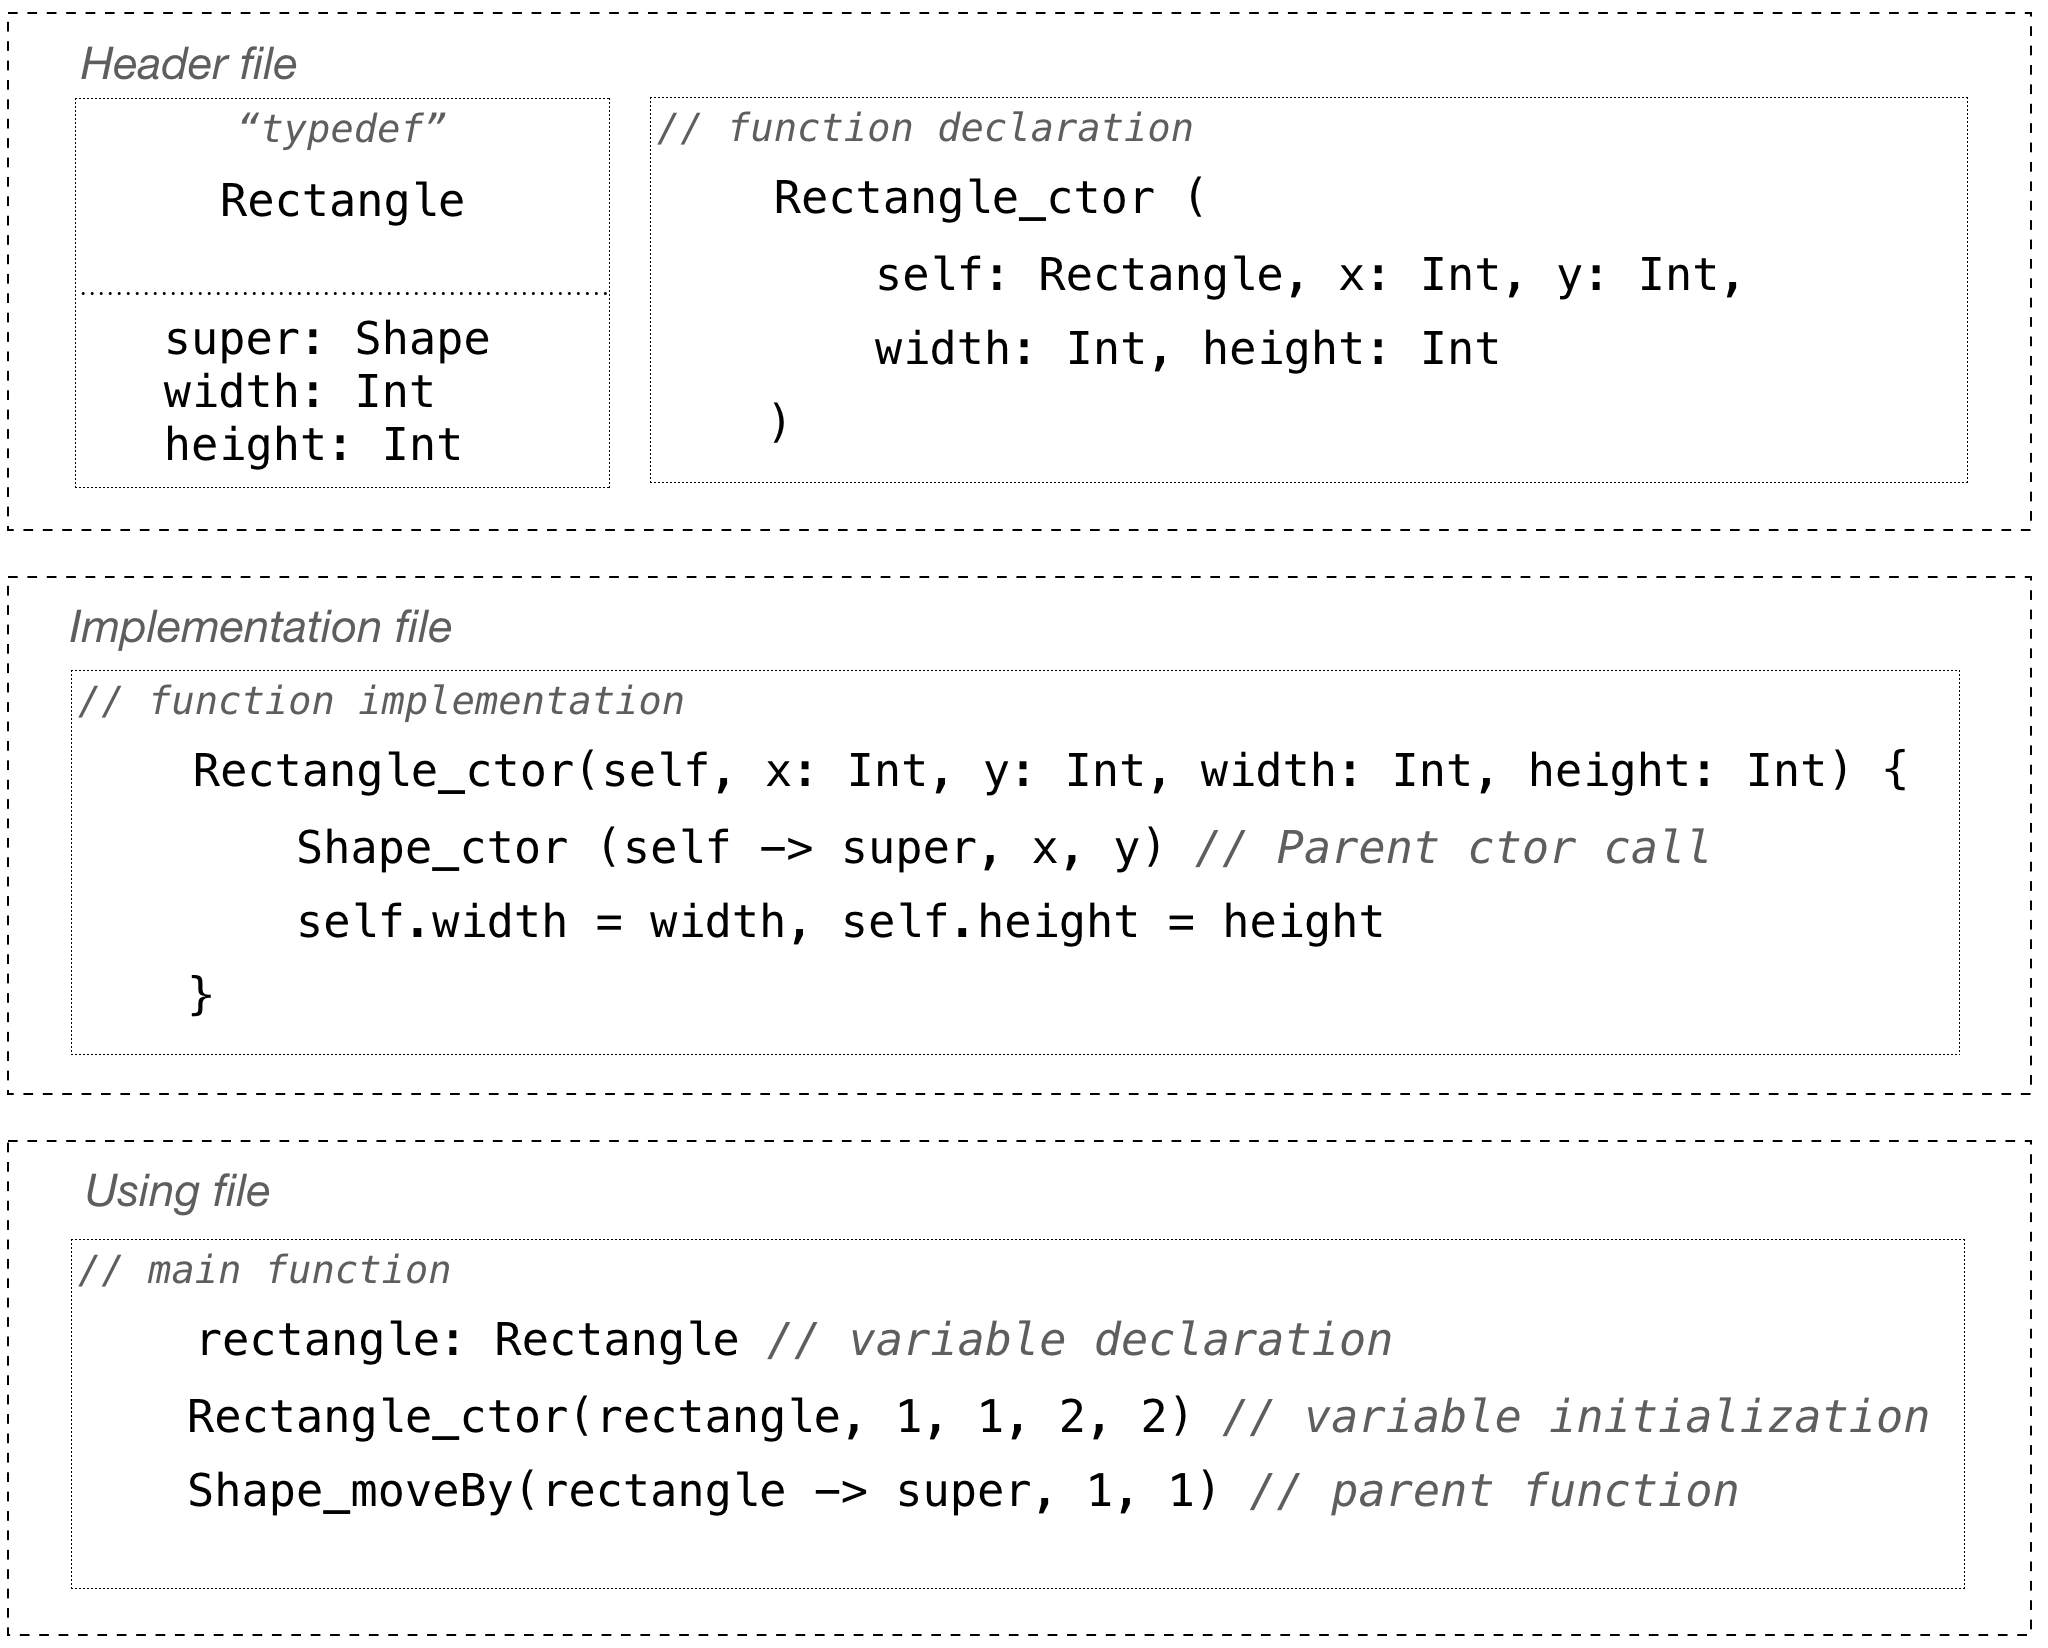
\includegraphics[width=\linewidth]{C_inh_scheme.png}
    \caption{Inheritance in C}
    \label{fig:C_inh_scheme}
\end{figure}

\subsubsection{Encapsulation}
In this thesis, encapsulation in the sense of access modifiers is not necessary to port object-oriented programs into C, as all the needed access checks are performed during generation of AST.

\subsubsection{Polymorphism}
Polymorphism implies the use of the common interface by similar classes, which is a much harder task than anything described above, as it cannot possibly be implemented without auxiliary constructs such as C++ virtual tables. 
Here, virtual tables are structures where pointers to ``virtual'' functions are declared. 
Consider the class as mentioned earlier Shape, with added functions area() and draw() that would calculate the shape area and draw the shape, respectively. 
Of course, it is not possible to calculate an area of an abstract shape or to draw an abstract shape. Thus these functions will be, in C++ terms, pure virtual, that is, required to be implemented by Shape descendants. On the Fig \ref{fig:C_UML} we can see the UML diagram of Shape along with Rectangle and Circle derived from it.

\begin{figure}[h!]
    \centering
    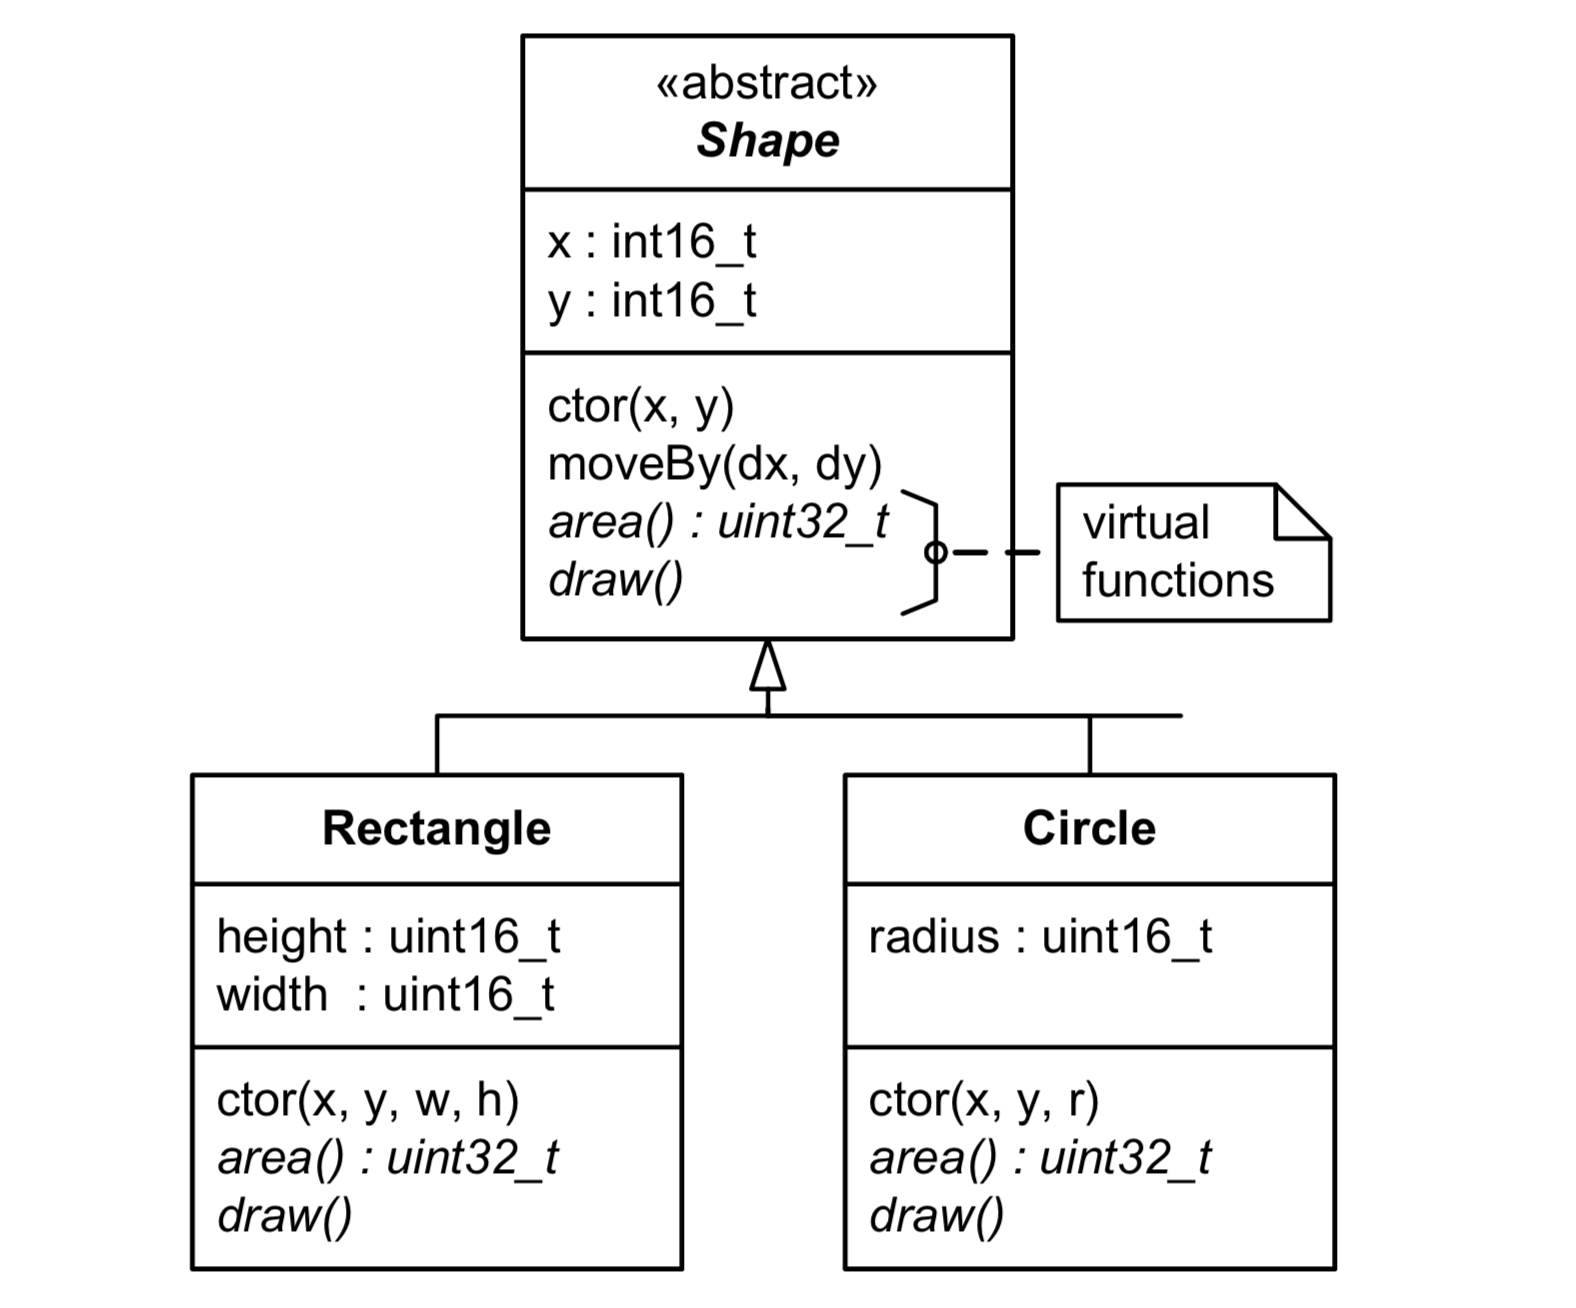
\includegraphics[width=\linewidth]{C_UML.png}
    \caption{Polymorphism in C, UML}
    \label{fig:C_UML}
\end{figure}

\subsection{Class declaration}
Consider the class Shape written in SLang:
\begin{lstlisting}[morekeywords={unit, end, is}, caption={Class declaration in Slang}, label={lst:Slang_class_decl}]
unit Shape 
    x: Int
    y: Int

    moveBy(dx: Int, dy: Int) is
        x += dx
        y += dy
    end moveBy
end
\end{lstlisting}

On the figure \ref{fig:C_class_decl_scheme} the declaration of the aforementioned class is schematically described. Declaration of the type and its methods is placed into the separate header file, and the type itself is declared using ``typedef struct''. In the associated source file the class methods are implemented. Methods use a pointer to a class object as the first argument to work with it. On the scheme, they are denoted as ``self''. Thus the object creation is creating a variable of the type of our class, and method call is performed by calling an associated function and passing the pointer to the object as the first parameter. The full Listing \ref{lst:C_class_decl} is available in the chapter \ref{chap:application}.

\begin{figure}[h!]
    \centering
    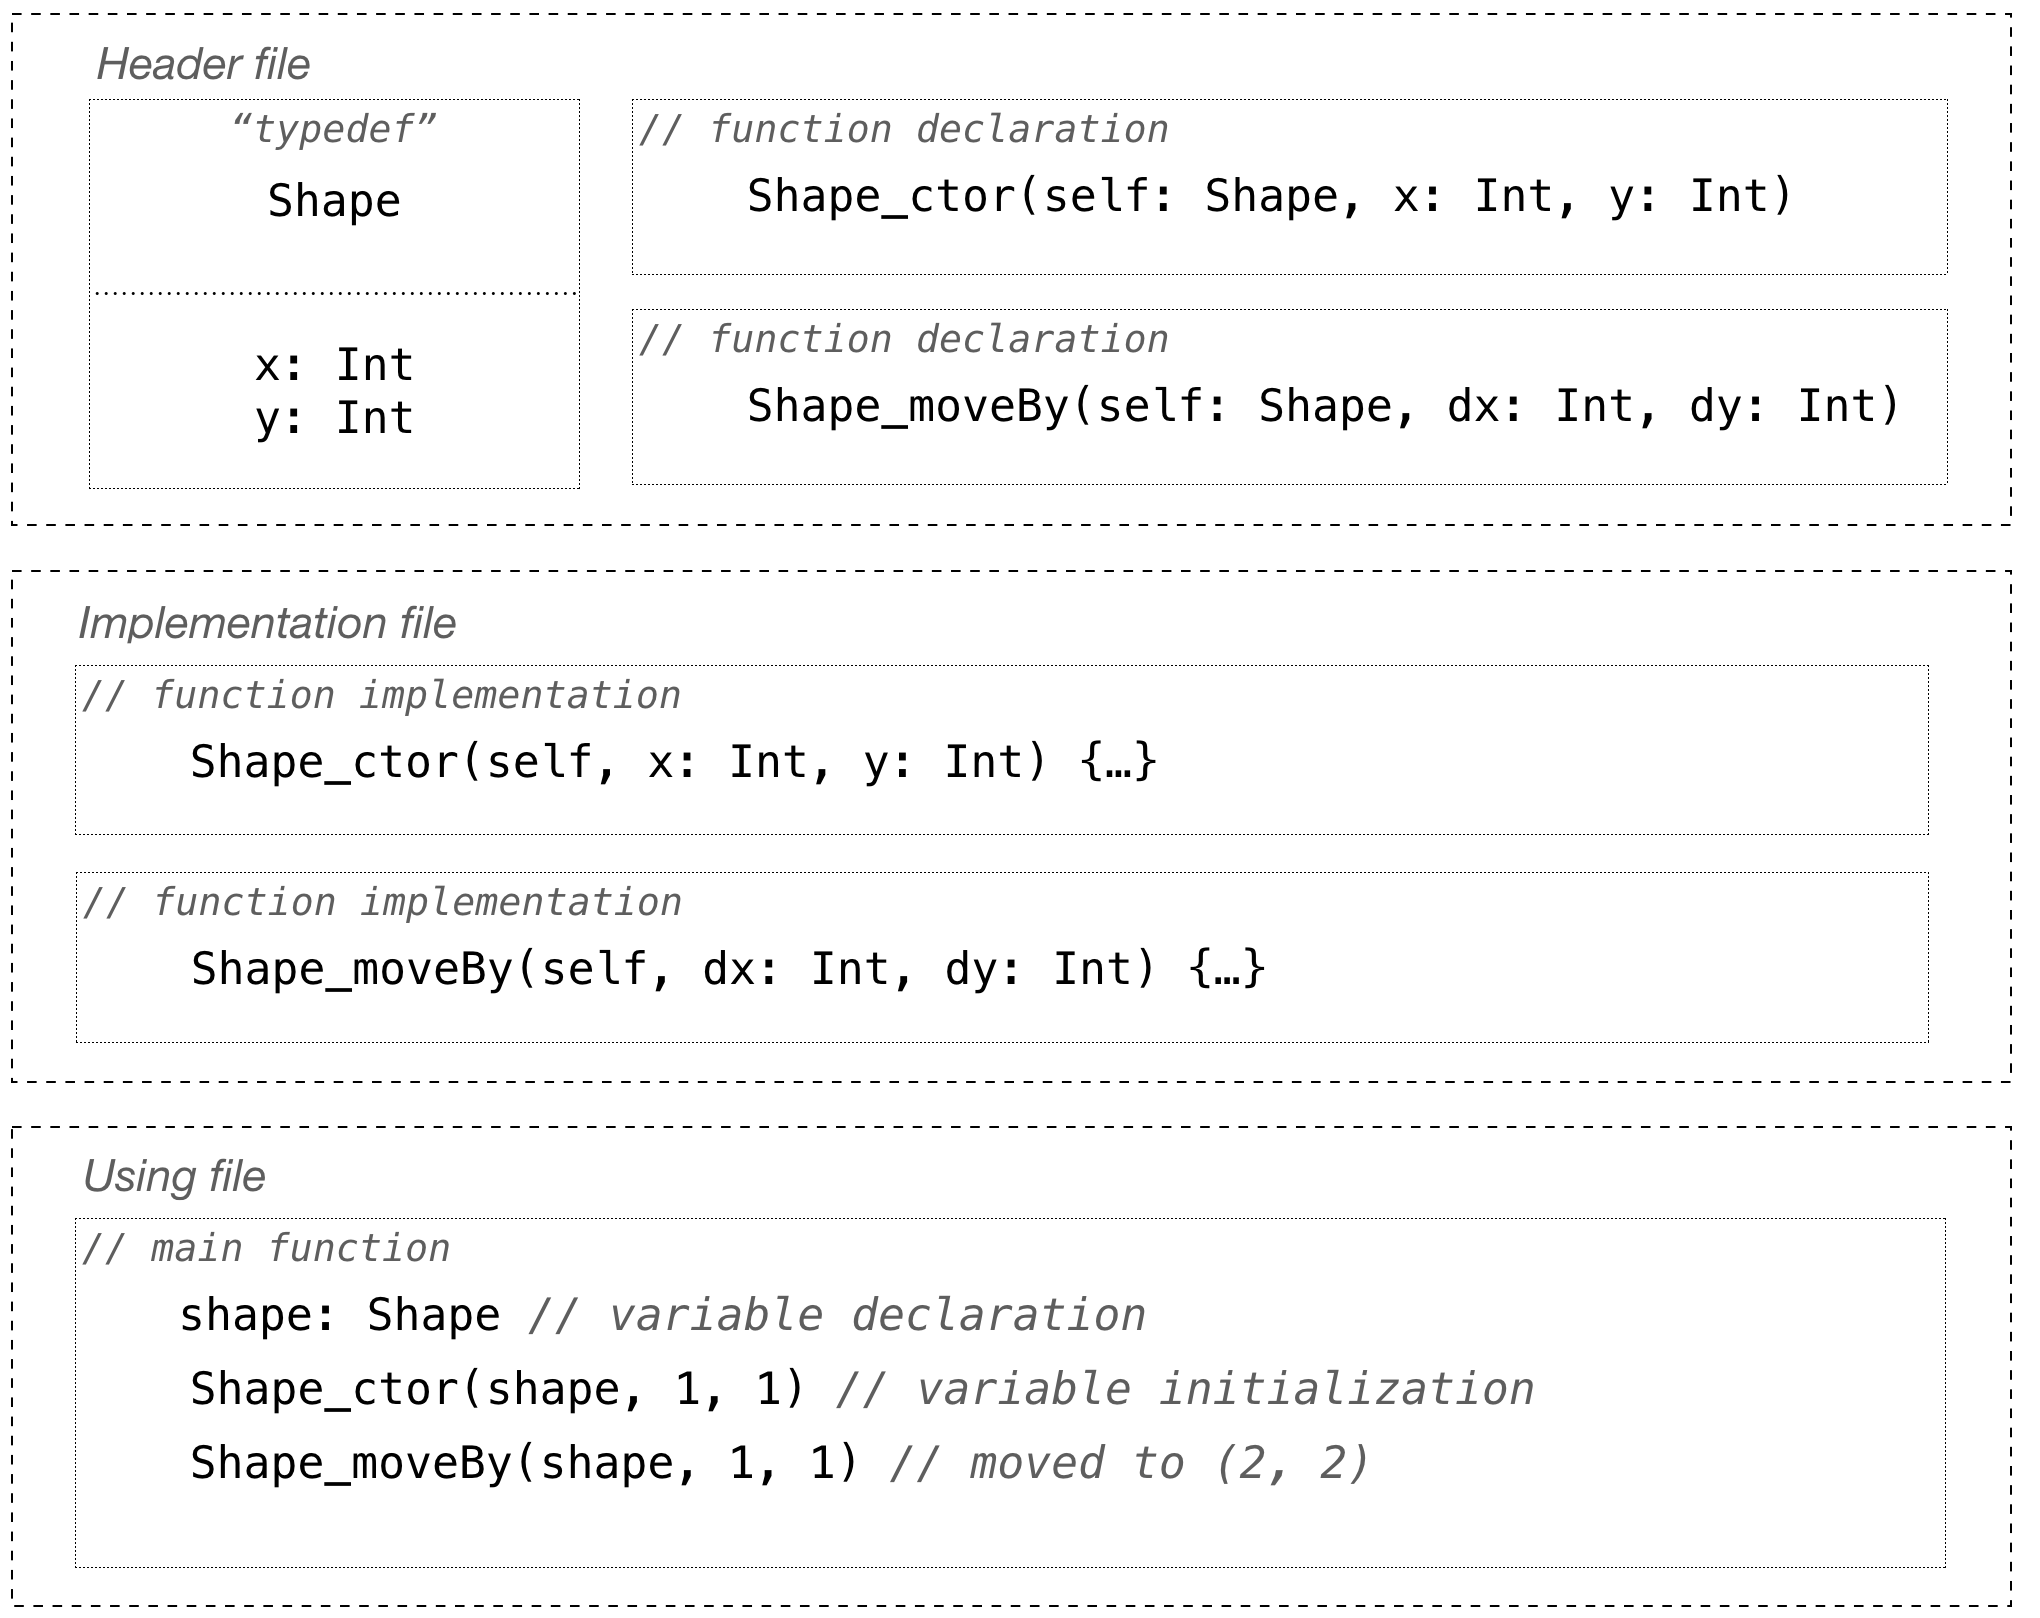
\includegraphics[width=\linewidth]{C_class_decl_scheme.png}
    \caption{Class declaration in C}
    \label{fig:C_class_decl_scheme}
\end{figure}


\subsection{Virtual table and Virtual pointer}
To implement the mechanism of virtual functions, we need a virtual table (vtbl) and a virtual pointer (vptr), which is going to be a part of a class. Virtual table as implemented in C is going to be a structure aggregating pointers to functions that are supposed to be virtual, as follows in Fig \ref{fig:ShapeVtblAndDecl} а), or Listing \ref{lst:Shapt_virt_table}.

Virtual Pointer is a pointer to the Virtual Table of the class. It must be defined for every instance of the class, which is to be done via making it one of the class fields. For example, the inner structure of the shape class can be seen on the Fig \ref{fig:ShapeVtblAndDecl} b) or in Listing \ref{lst:Shapt_virt_pointer}:

\begin{figure}[h!]
    \centering
    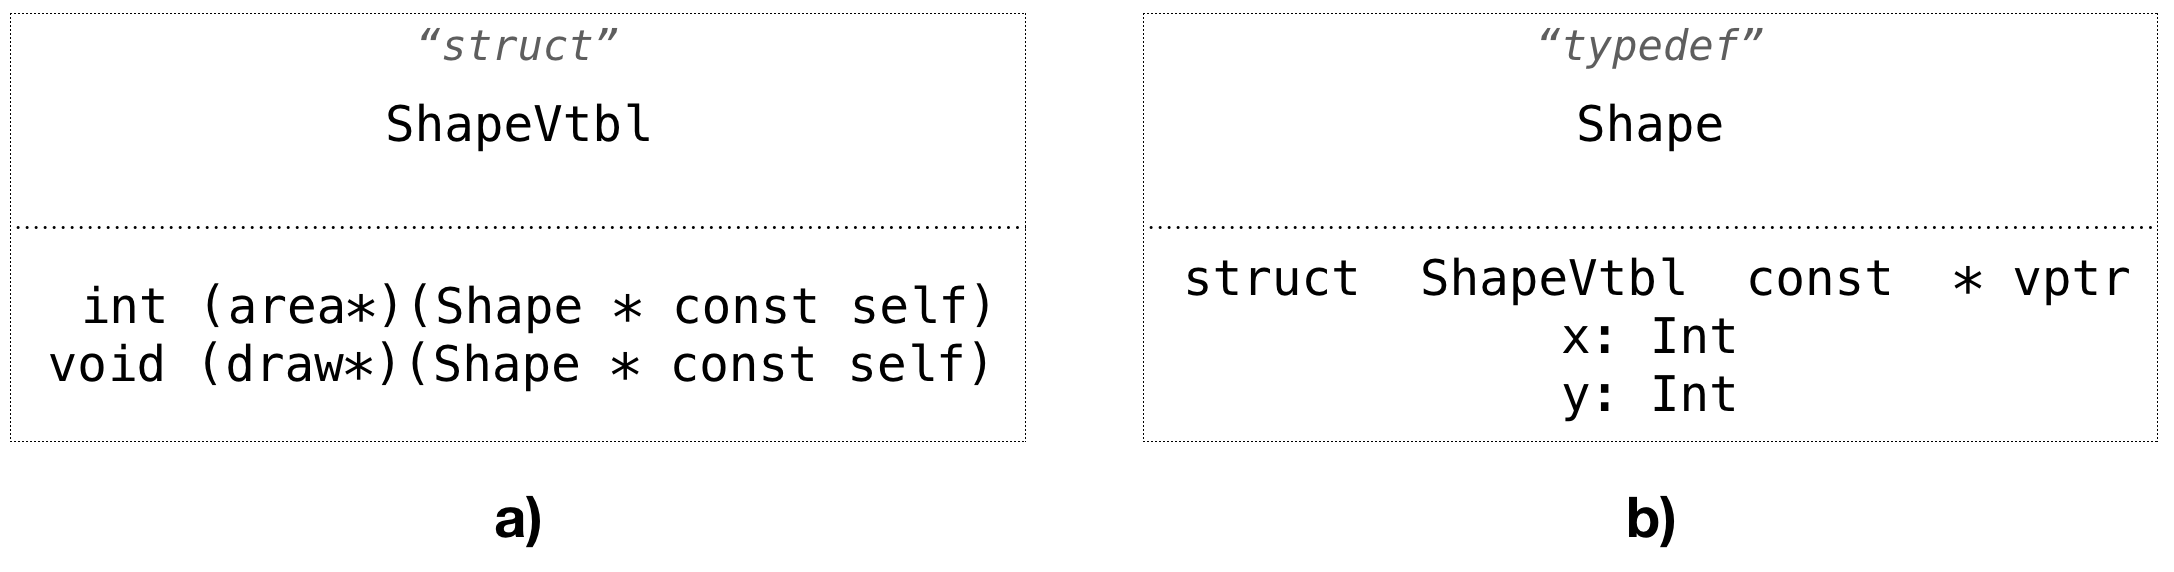
\includegraphics[width=\linewidth]{ShapeVtblAndDecl.png}
    \caption{ShapeVtbl struct declaration: a and Shape class declaration: b)}
    \label{fig:ShapeVtblAndDecl}
\end{figure}


\subsection{Setting the vptr in the Constructor}
For every instance of the class, its virtual pointer must be set to the corresponding virtual table, preferably on object creation, which implies that class’ constructor would be a perfect place to do that, Listing \ref{lst:Shape_vtbl_vptr}, Figure \ref{fig:Shape_vtbl_vptr_assignment}. 

\begin{figure}[h!]
    \centering
    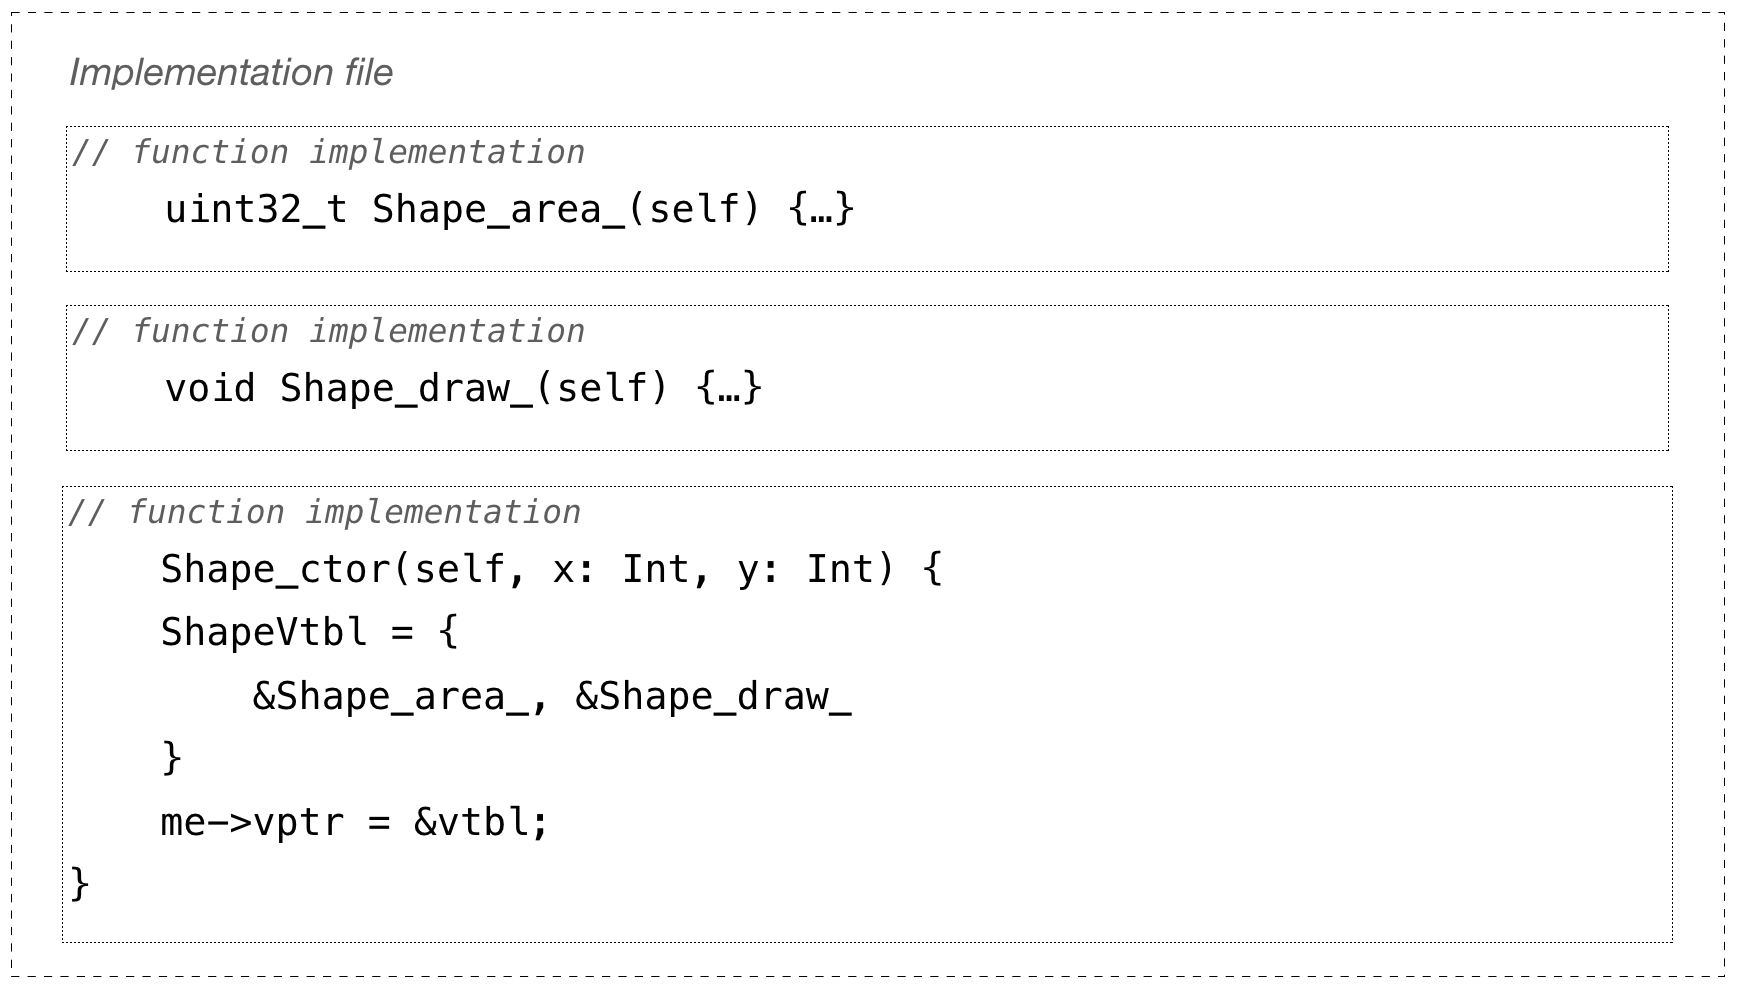
\includegraphics[width=\linewidth]{Shape_vtbl_vptr_assignment.png}
    \caption{Defining the virtual table and initializing the virtual pointer}
    \label{fig:Shape_vtbl_vptr_assignment}
\end{figure}

If a reasonable implementation of a virtual function cannot be provided in a class, which happens in case of abstract classes, implementations should ensure they interrupt the runtime (as they would not work in object-oriented languages in any case) with smart use of asserts, Listing \ref{lst:Pure_virt}.

\subsection{Inheriting the vtbl and Overriding the vptr in the Subclasses}
Due to the way inheritance is implemented, vptr is inherited automatically if present in the base class, by all subclasses at all levels, so for polymorphic classes, the principle of attribute inheritance works automatically.

Nevertheless, for every specififc subclass vptr needs to be reassigned to the respective vtbl, which also is to happen inside a constructor. For instance, consider the constructor of the Rectangle class, derived from Shape:

\begin{lstlisting}[caption={Overriding the vtbl and vptr in the subclass Rectangle}, label=lst:Overriding_vtbl_vptr]
/* Rectangle's class implementations of its virtual functions*/ 
static uint32_t Rectangle_area_( * const me);
static void Rectangle_draw_( * const me);
/* constructor */
void Rectangle_ctor(Rectangle * const me, int16_t x, int16_t y,
uint16_t width, uint16_t height)
{
    static struct ShapeVtbl const vtbl = { 
        /* vtbl of the Rectangle class */
        &Rectangle_area_,
        &Rectangle_draw_
    };
    Shape_ctor(&me->super, x, y); /*call the superclass' ctor*/
    me->super.vptr = &vtbl; /* override the vptr */
    me->width = width;
    me->height = height; 
}
\end{lstlisting} 

First of all, to initialize the me->super member, which is necessarily a subobject of the type of the superclass, the Shape constructor is invoked. There, the vptr is set to Shape’s vtbl. However, in the next statement it is reassigned to the Rectangle’s vtbl, so the vptr is overridden.

To fit into the vtbl, all implementations of virtual functions that are made for a subclass must precisely match signatures predefined earlier in the superclass. For example, the implementation Rectangle\_area\_() takes the pointer “me” of type Shape*, not Rectangle*, exactly for this reason, so in the actual implementation, an explicit downcast should be performed, as in Listing \ref{lst:Downcasting_me}:

\begin{lstlisting}[caption={Explicit downcasting of the “me” pointer}, label=lst:Downcasting_me]
static uint32_t Rectangle_area_(Shape * const me) {
    Rectangle * const me_ = (Rectangle *)me; /* explicit downcast */
    return (uint32_t)->width * (uint32_t)me_->height;
}
\end{lstlisting}

\subsection{Virtual Call}
With the following infrastructure of Virtual Tables and Virtual Pointers, the virtual call (late binding) can be implemented like in the example below:
\begin{lstlisting}[]
uint32_t Shape_area(Shape * const me) {
    return (*me->vptr->area)(me);
}
\end{lstlisting}

The virtual call works by first de-referencing the vtbl of the object to find the corresponding vtbl and only then calling the appropriate implementation from this vtbl via a pointer-to-function. The figure \ref{fig:virtual_call_mech} illustrates this process.

\begin{figure}[h!]
    \centering
    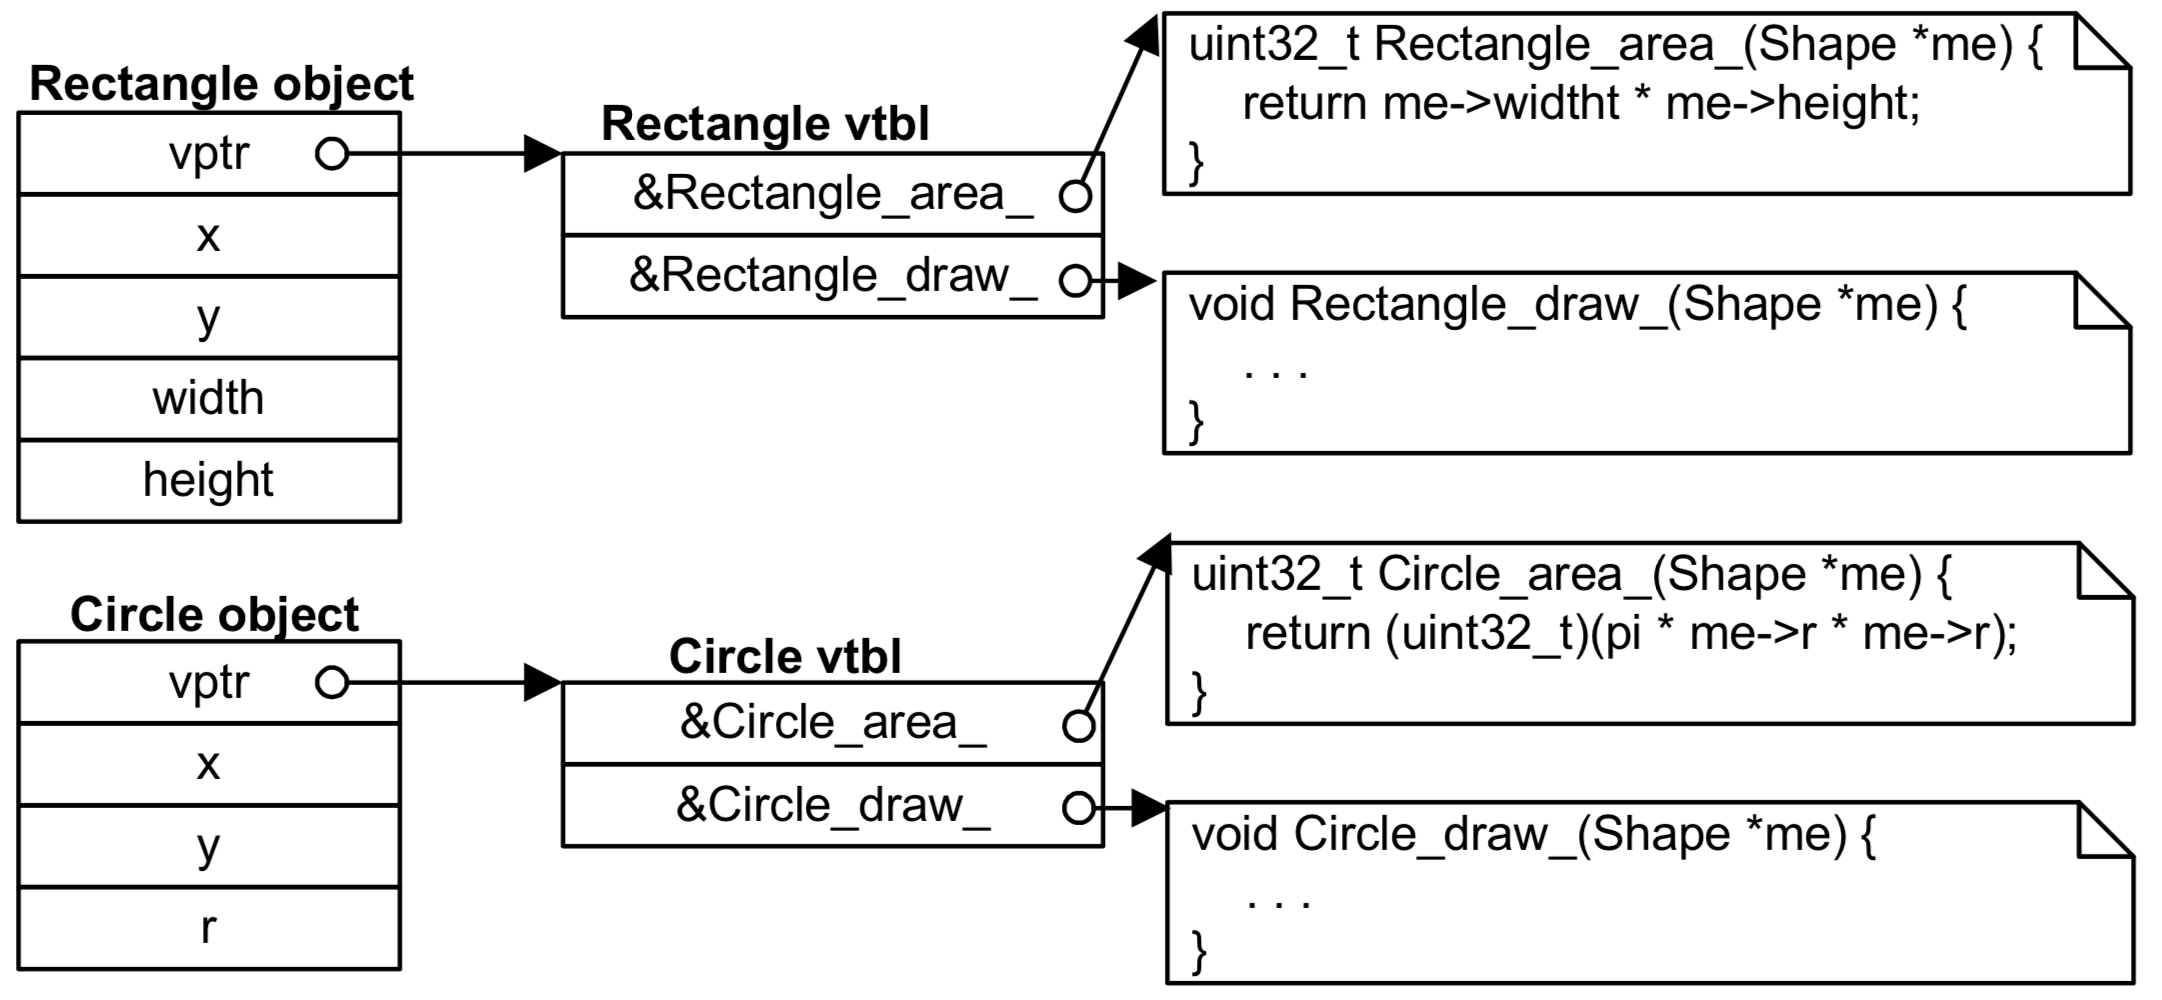
\includegraphics[width=\linewidth]{virtual_call_mech.png}
    \caption{Virtual call mechanism for Rectangles and Circles}
    \label{fig:virtual_call_mech}
\end{figure}

 
% Referencing other chapters \ref{chap:lr}, \ref{chap:met}, \ref{chap:impl}, \ref{chap:eval} and \ref{chap:conclusion}
